\documentclass[11pt, a4paper]{article}
\usepackage{pdfpages}
\usepackage{parallel}
\usepackage[T2A]{fontenc}
\usepackage{ucs}
\usepackage[utf8x]{inputenc}
\usepackage[polish,english,russian]{babel}
\usepackage{hyperref}
\usepackage{rotating}
\usepackage[inner=2cm,top=1.8cm,outer=2cm,bottom=2.3cm,nohead]{geometry}
\usepackage{listings}
\usepackage{graphicx}
\usepackage{wrapfig}
\usepackage{longtable}
\usepackage{indentfirst}
\usepackage{array}
\usepackage{tikzsymbols}
\usepackage{soul}
\usepackage[ruled,vlined]{algorithm2e}
%\counterwithout{figure}{section} 

\usepackage{url}
\makeatletter
\g@addto@macro{\UrlBreaks}{\UrlOrds}
\makeatother

\newcolumntype{P}[1]{>{\raggedright\arraybackslash}p{#1}}
\frenchspacing
\usepackage{fixltx2e} %text sub- and superscripts
\usepackage{icomma} % коскі ў матэматычным рэжыме
\PreloadUnicodePage{4}

\newcommand{\longpage}{\enlargethispage{\baselineskip}}
\newcommand{\shortpage}{\enlargethispage{-\baselineskip}}

\def\switchlang#1{\expandafter\csname switchlang#1\endcsname}
\def\switchlangbe{
\let\saverefname=\refname%
\def\refname{Літаратура}%
\def\figurename{Іл.}%
}
\def\switchlangen{
\let\saverefname=\refname%
\def\refname{References}%
\def\figurename{Fig.}%
}
\def\switchlangru{
\let\saverefname=\refname%
\let\savefigurename=\figurename%
\def\refname{Литература}%
\def\figurename{Рис.}%
}

\hyphenation{admi-ni-stra-tive}
\hyphenation{ex-pe-ri-ence}
\hyphenation{fle-xi-bi-li-ty}
\hyphenation{Py-thon}
\hyphenation{ma-the-ma-ti-cal}
\hyphenation{re-ported}
\hyphenation{imp-le-menta-tions}
\hyphenation{pro-vides}
\hyphenation{en-gi-neering}
\hyphenation{com-pa-ti-bi-li-ty}
\hyphenation{im-pos-sible}
\hyphenation{desk-top}
\hyphenation{elec-tro-nic}
\hyphenation{com-pa-ny}
\hyphenation{de-ve-lop-ment}
\hyphenation{de-ve-loping}
\hyphenation{de-ve-lop}
\hyphenation{da-ta-ba-se}
\hyphenation{plat-forms}
\hyphenation{or-ga-ni-za-tion}
\hyphenation{pro-gramming}
\hyphenation{in-stru-ments}
\hyphenation{Li-nux}
\hyphenation{sour-ce}
\hyphenation{en-vi-ron-ment}
\hyphenation{Te-le-pathy}
\hyphenation{Li-nux-ov-ka}
\hyphenation{Open-BSD}
\hyphenation{Free-BSD}
\hyphenation{men-ti-on-ed}
\hyphenation{app-li-ca-tion}

\def\progref!#1!{\texttt{#1}}
\renewcommand{\arraystretch}{2} %Іначай формулы ў матрыцы зліпаюцца з лініямі
\usepackage{array}

\def\interview #1 (#2), #3, #4, #5\par{

\section[#1, #3, #4]{#1 -- #3, #4}
\def\qname{LVEE}
\def\aname{#1}
\def\q ##1\par{{\noindent \bf \qname: ##1 }\par}
\def\a{{\noindent \bf \aname: } \def\qname{L}\def\aname{#2}}
}

\def\interview* #1 (#2), #3, #4, #5\par{

\section*{#1\\{\small\rm #3, #4. #5}}
\ifx\ParallelWhichBox\undefined%
    \addcontentsline{toc}{section}{#1, #3, #4}%
\else%
\ifnum\ParallelWhichBox=0%
    \addcontentsline{toc}{section}{#1, #3, #4}%
\fi\fi%

\def\qname{LVEE}
\def\aname{#1}
\def\q ##1\par{{\noindent \bf \qname: ##1 }\par}
\def\a{{\noindent \bf \aname: } \def\qname{L}\def\aname{#2}}
}

\newcommand{\interviewfooter}[1]{
\vskip 1em
\noindent \textit{#1}
}

\switchlang{en}
\begin{document}

\title{1980 "--- Contour UniMouse}
\date{}
\author{~}
\maketitle
\selectlanguage{english}

The UniMouse computer mouse was released by Contour Design, a company that specializes exclusively in ergonomic manipulators, for Apple iMac computers as a replacement for the bundled Apple USB mouse, known as the "puck" because of its round shape. The Apple USB mouse was criticized by many for its poor ergonomics, and a year after it hit the market, an alternative was released from one of the leaders in ergonomic cursor controls \cite{pressrelease}.

\begin{figure}[h]
   \centering
    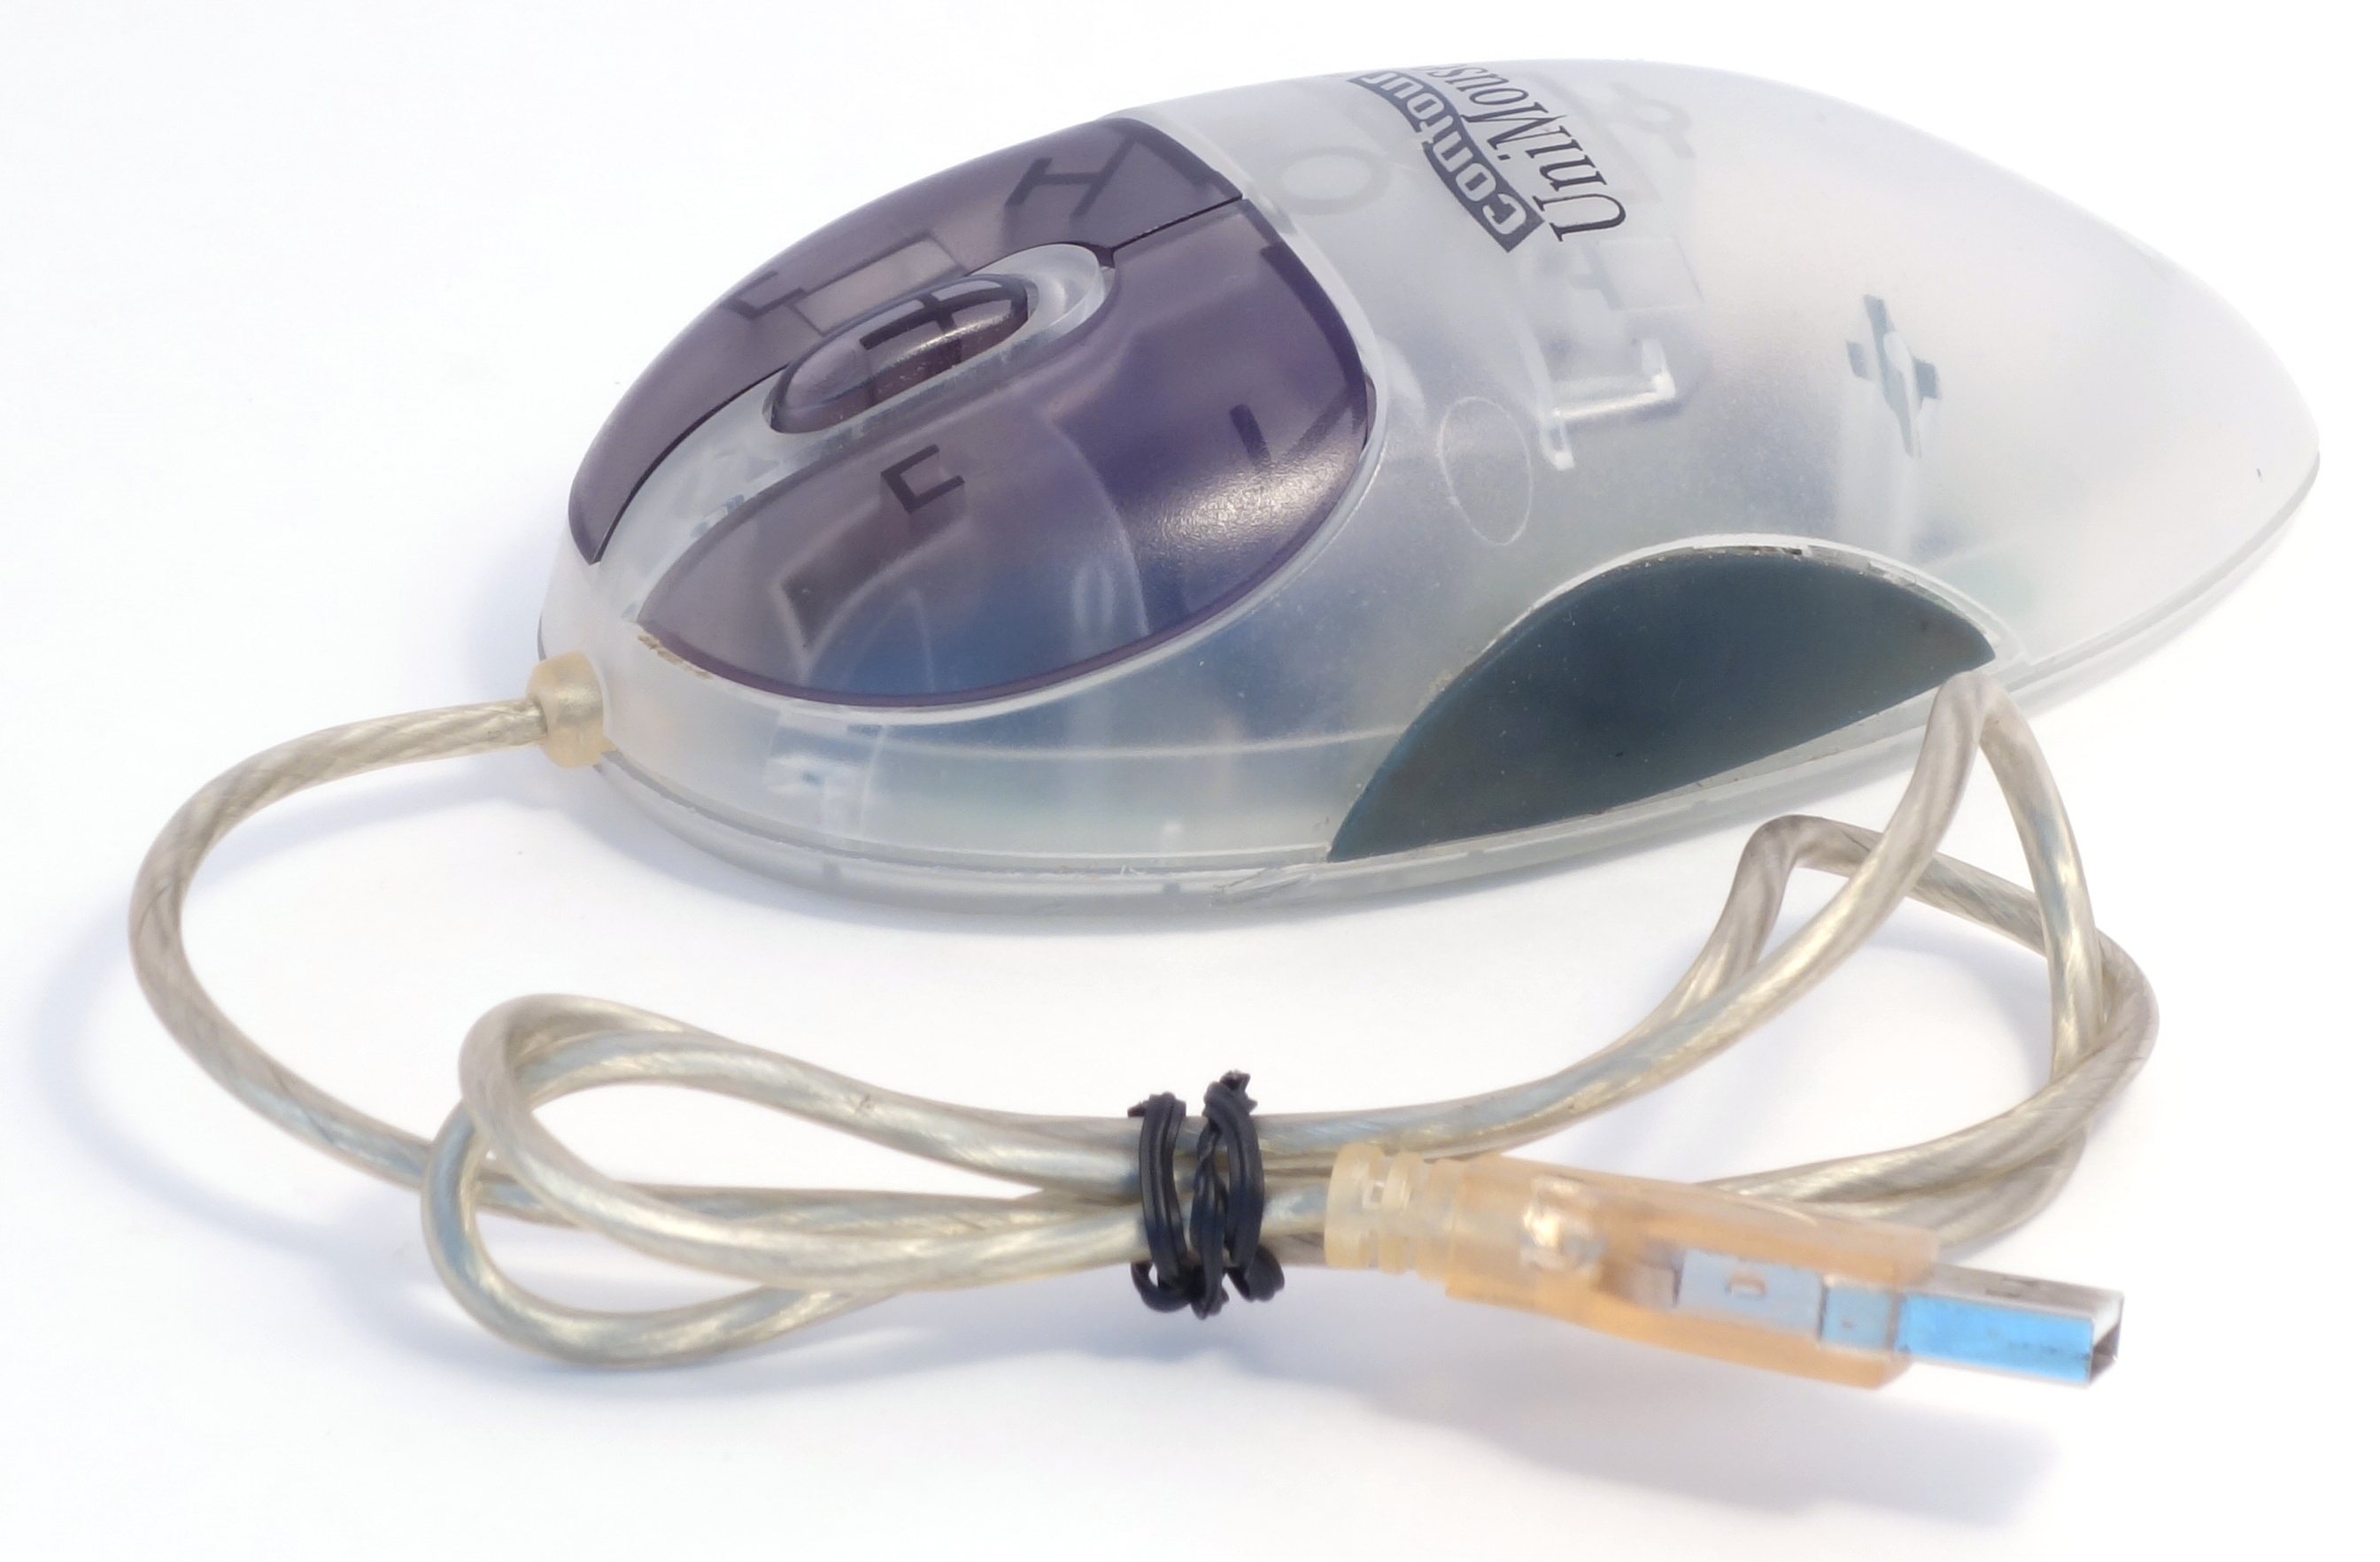
\includegraphics[scale=0.53]{1999_contour_unimouse/pic_30.jpg}
    \caption{Contour UniMouse}
    \label{fig:ContourUniMousePic}
\end{figure}

The mouse has a translucent body that shows through the circuit board \ref{fig:ContourUniMouseTopAndBottom}, decorated with tinted buttons and the name of the mouse printed on top. Two large buttons are located in the front part of the body. Between them there is a convex third button, visually stylized as a scroll wheel. The clear plastic bottom of the mouse looks quite traditional, including low-friction feet and a latch ring to remove the ball for cleaning. Two rubber pads on the sides of the body are there for a more comfortable grip.

\begin{figure}[h]
    \centering
    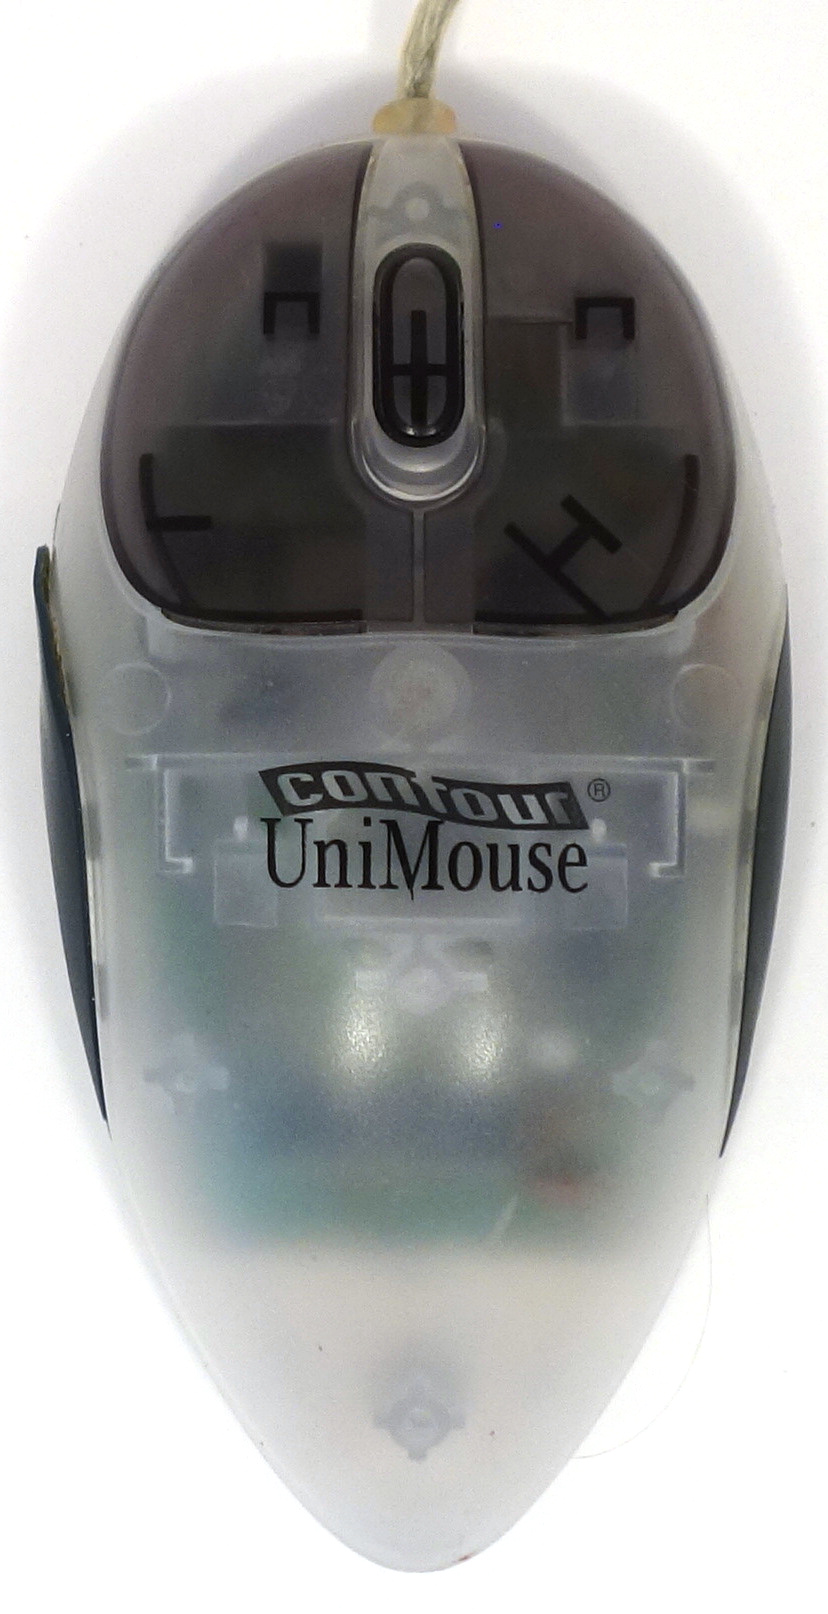
\includegraphics[scale=0.48]{1999_contour_unimouse/top_30.jpg}
    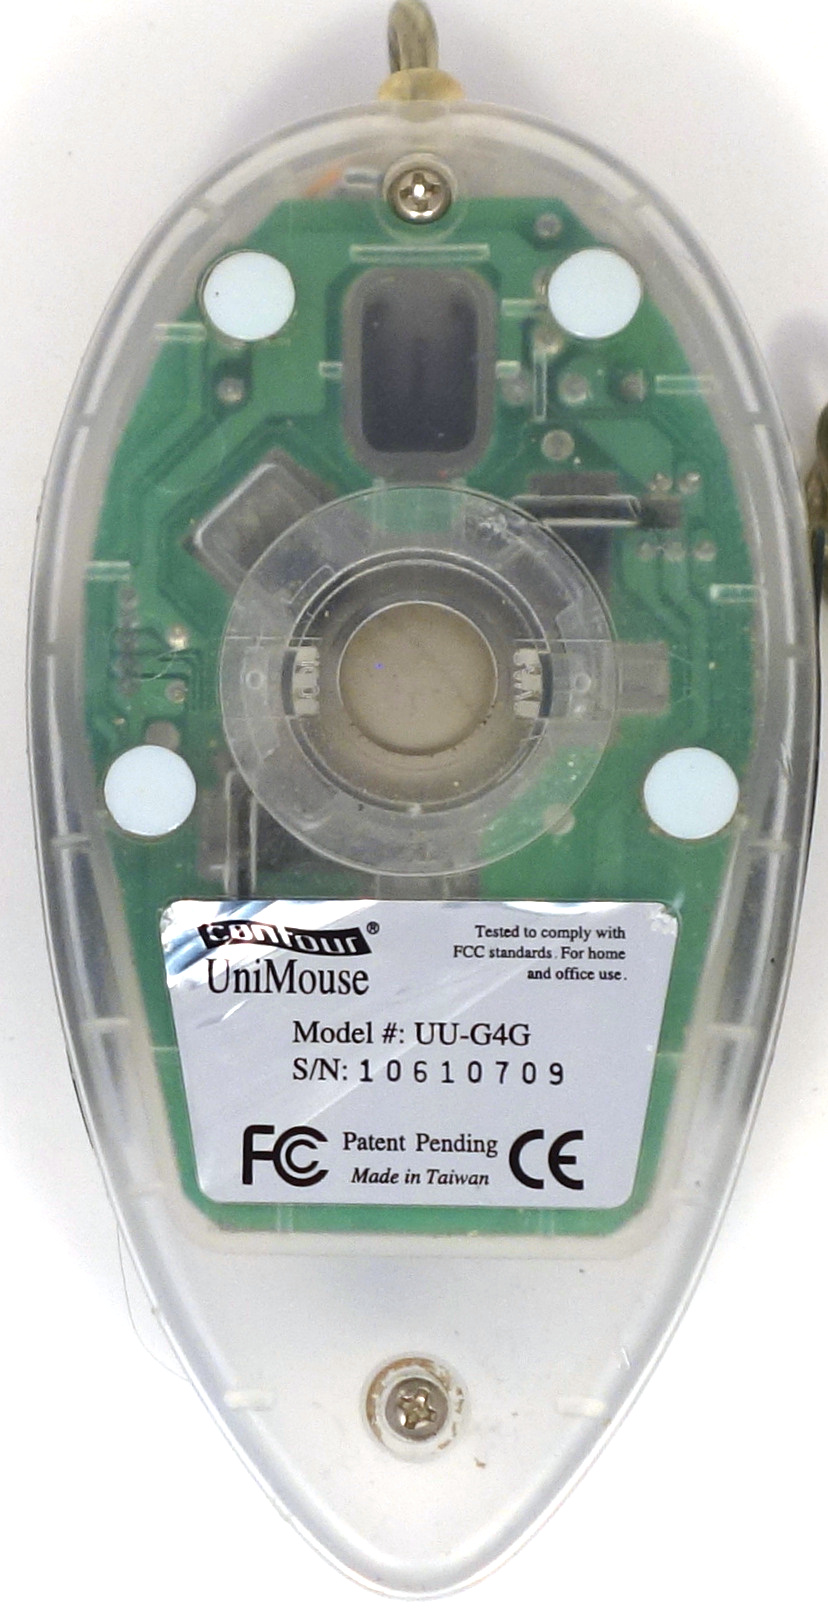
\includegraphics[scale=0.48]{1999_contour_unimouse/bottom_30.jpg}
    \caption{Contour UniMouse, top and bottom views}
    \label{fig:ContourUniMouseTopAndBottom}
\end{figure}

The mouse had several color options for buttons, rubber pads, and printed name to match the iMac body design options \cite{web}.

The dimensions of the mouse (unlike the Apple USB mouse) are average, typical for mice of the late nineties (fig. \ref{fig:ContourUniMouseSize}).

\begin{figure}[h]
    \centering
    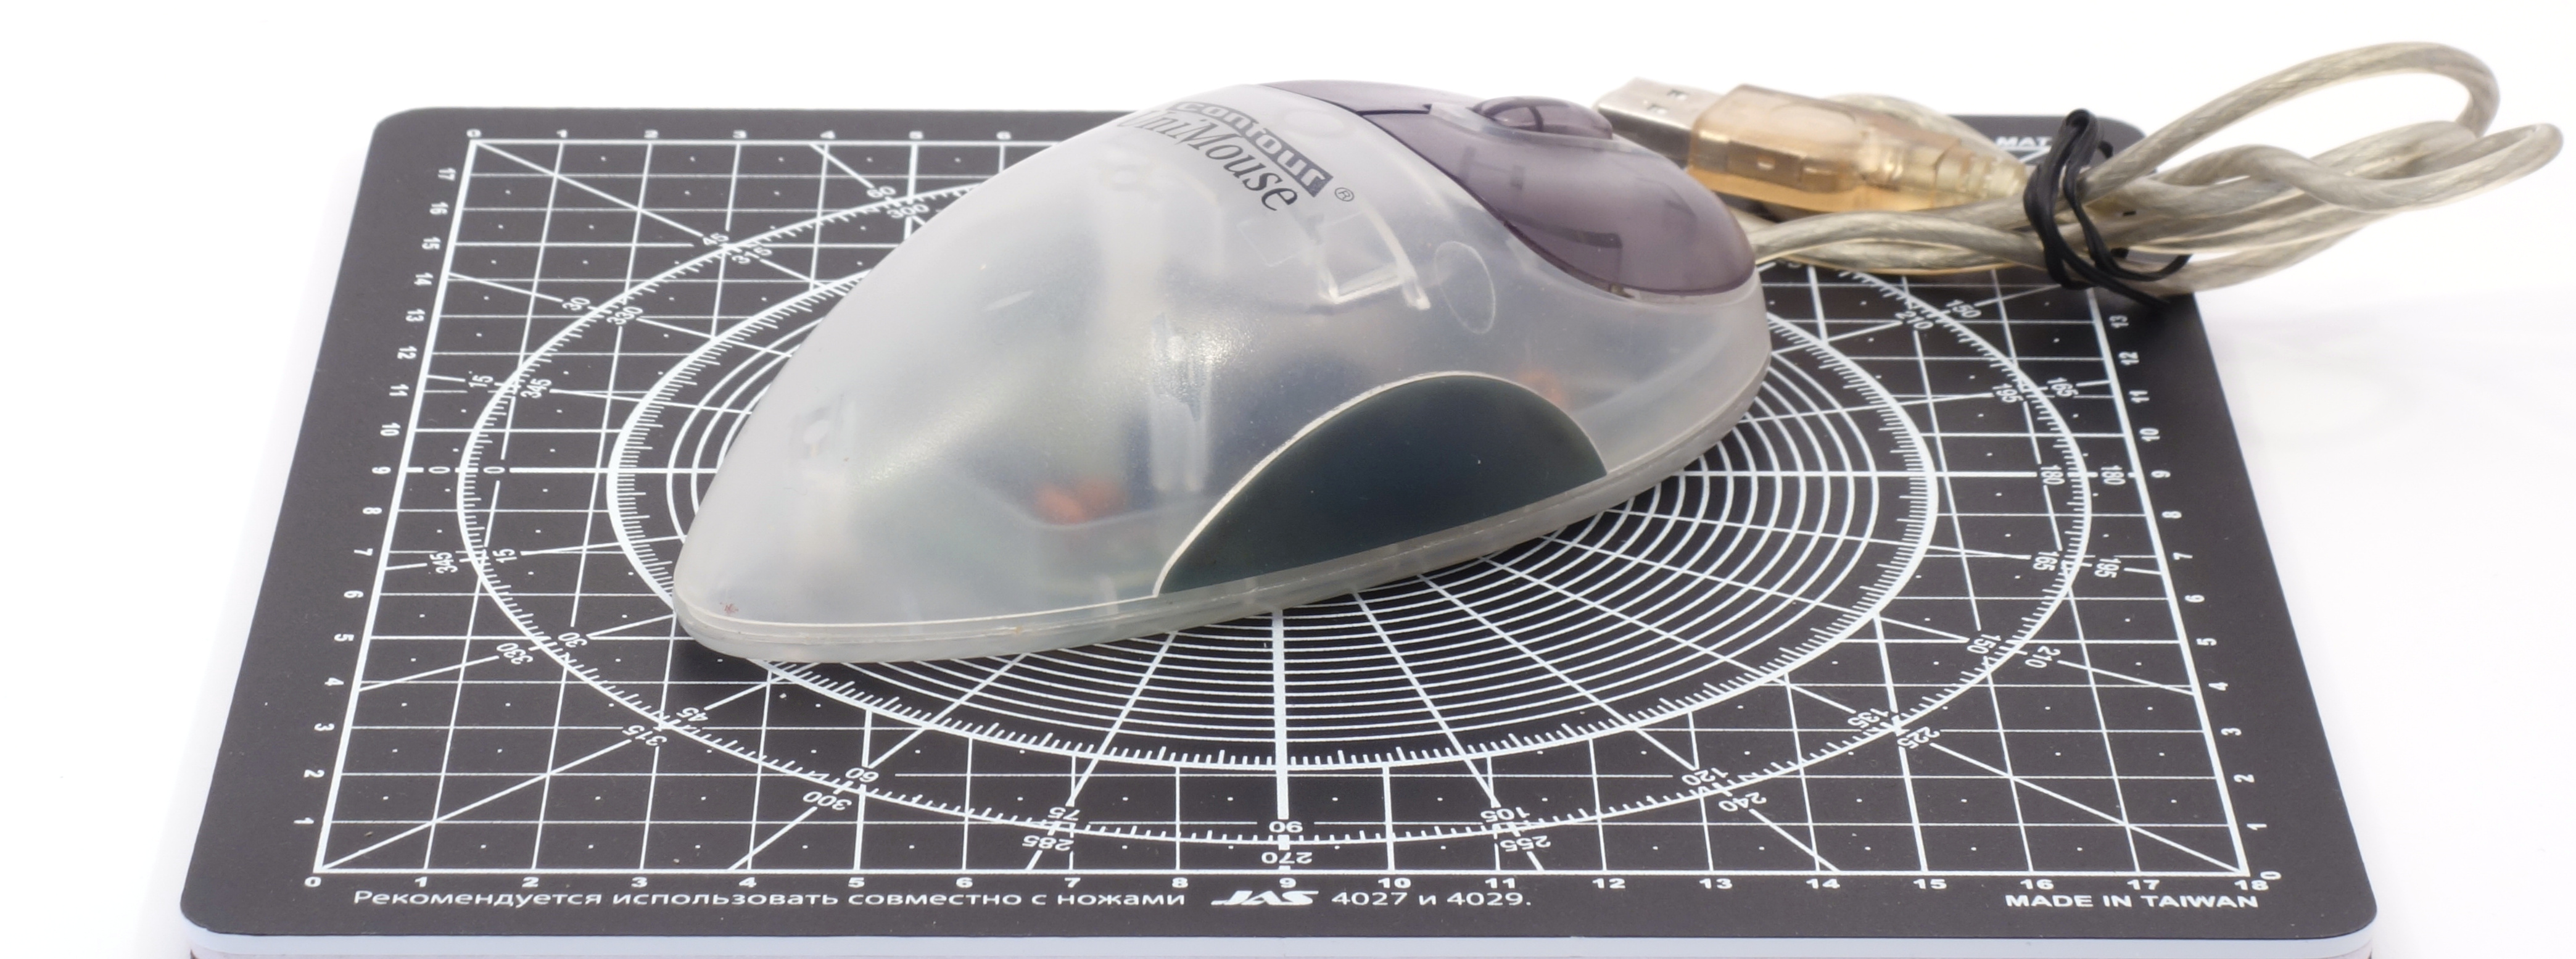
\includegraphics[scale=0.5]{1999_contour_unimouse/size_30.jpg}
    \caption{Contour UniMouse on a graduated pad with a grid step of 1~cm}
    \label{fig:ContourUniMouseSize}
\end{figure}

Due to the symmetry, the mouse is equally suitable for both left-handers and right-handers. Given the specialization of Contour Design, it is not surprising that the hand rests comfortably on the mouse (fig. \ref{fig:ContourUniMouseHand}).

\begin{figure}[h]
    \centering
    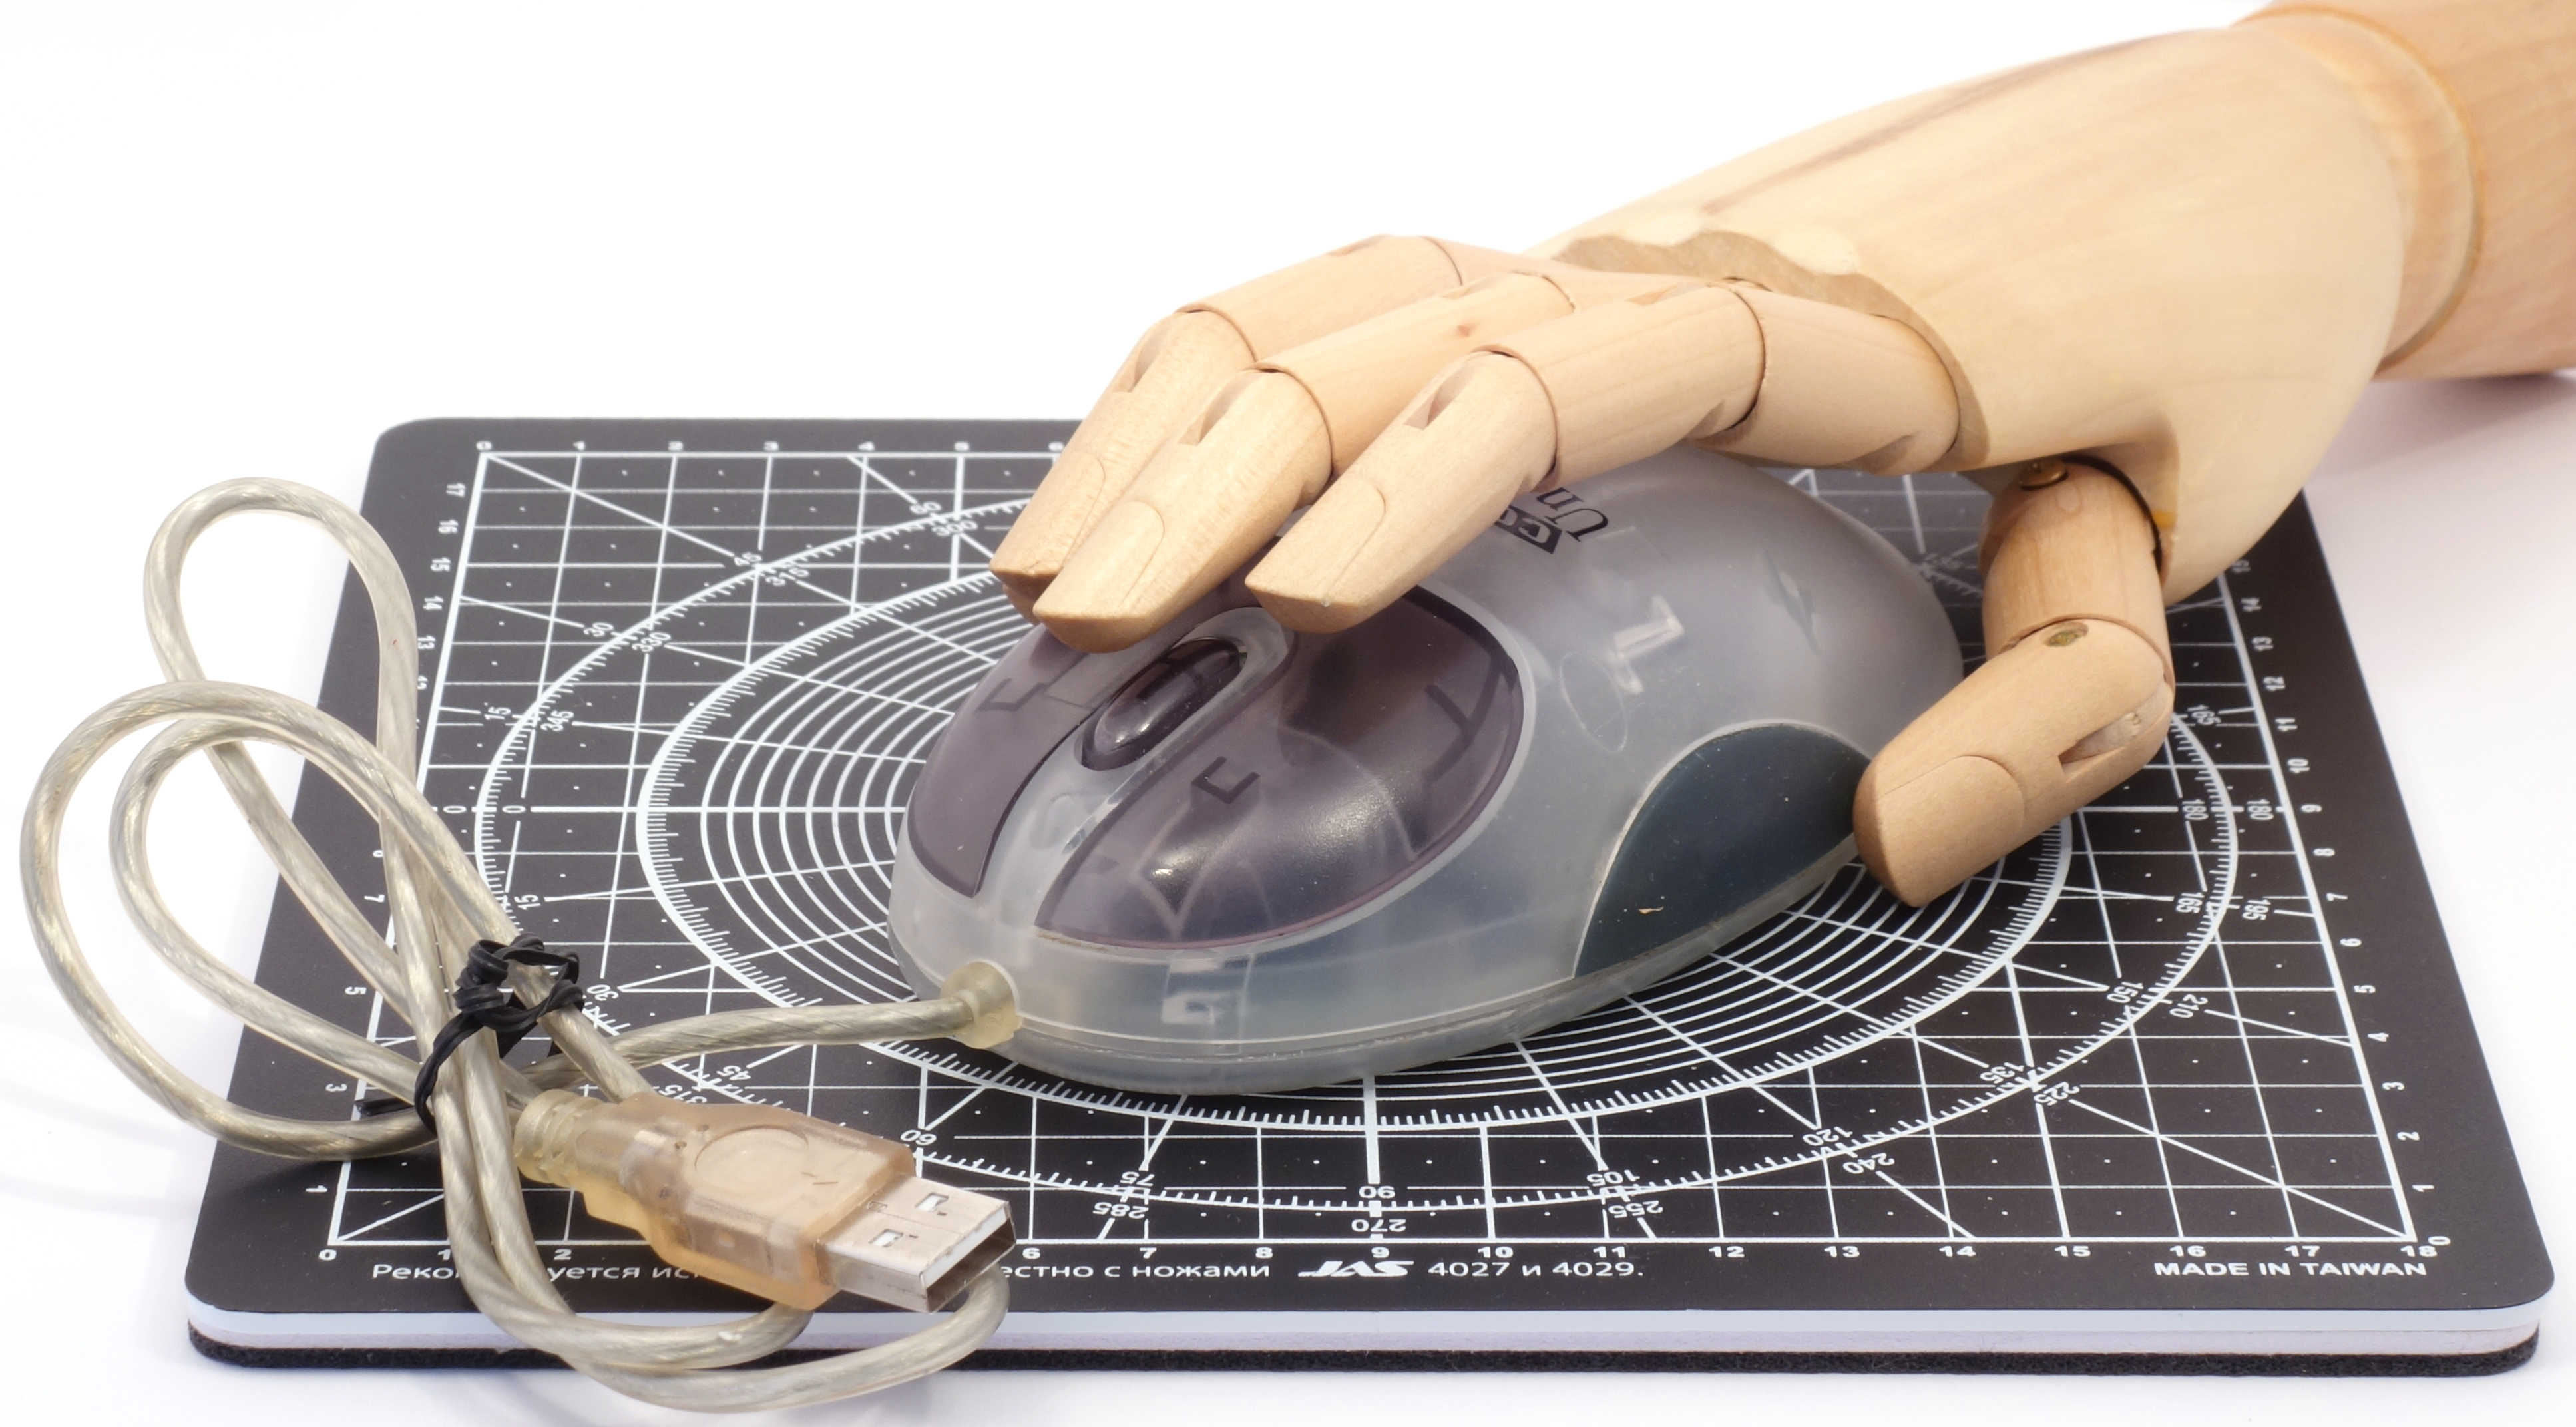
\includegraphics[scale=0.55]{1999_contour_unimouse/hand_30.jpg}
    \caption{Contour UniMouse with a human hand model}
    \label{fig:ContourUniMouseHand}
\end{figure}

A minor drawback mentioned in \cite{mactoday} is its relatively small area of the wrist support. The lack of a scroll wheel was compensated by software implementation: scrolling in four directions was carried out by moving the mouse when pressing the middle button. Obviously, this solution can hardly be called ideal: it is more difficult for the user than traditional scrolling, the button itself is less convenient, and besides, it is required to download a specially configured driver and/or additional software from the mouse manufacturer's website. However, in general, for the Apple platform, this mouse was a high-quality solution to compensate the Apple USB mouse problematic ergonomics, for which third-party manufacturers were even producing special overlay adapters that gave it a longer shape.

\begin{figure}[h]
    \centering
    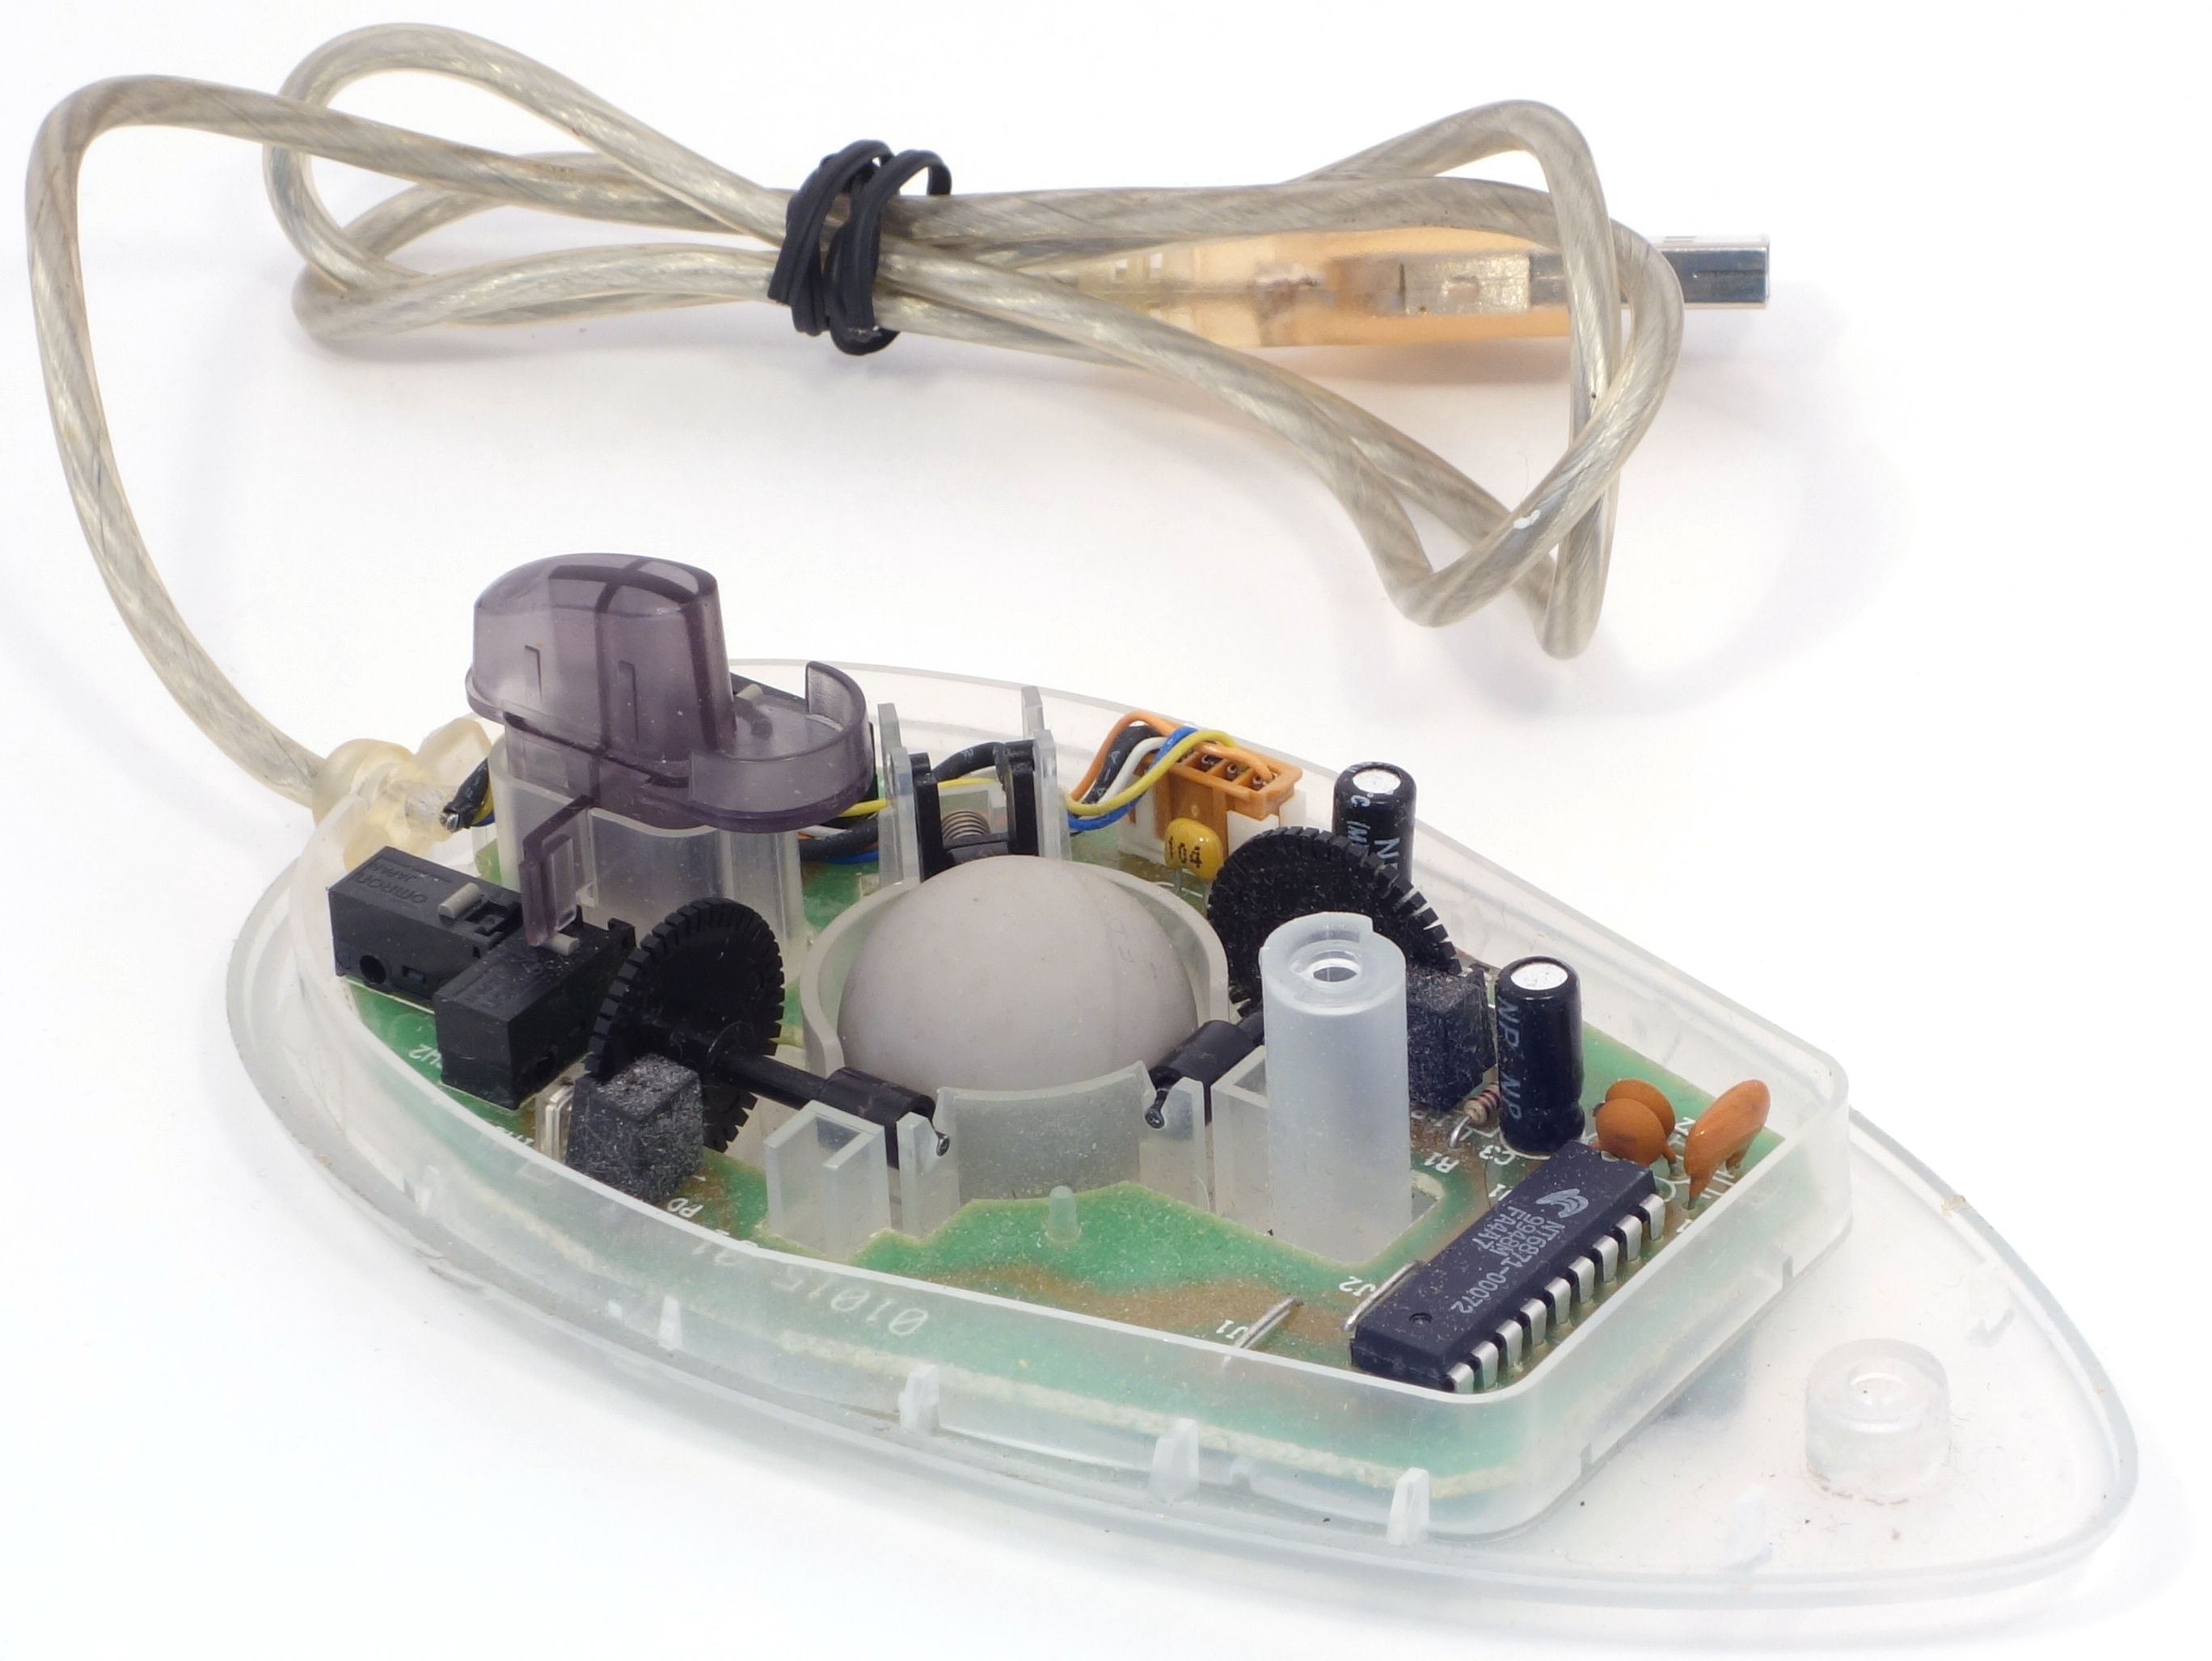
\includegraphics[scale=0.7]{1999_contour_unimouse/inside_30.jpg}
    \caption{Contour UniMouse disassembled}
    \label{fig:ContourUniMouseInside}
\end{figure}

The internals of this mouse are shown in fig. \ref{fig:ContourUniMouseInside}, which allows it to be classified as a traditional optomechanical design. The disc shape of the optical interrupter with teeth instead of slits is more typical among mice of the earlier period, however in this model the frequency of the teeth is markedly increased for greater resolution and corresponds to the frequency of the slits in the interrupters of other quality mice of the late nineties. At the same time, plastic is used as much as possible in the design, there are no expensive mechanical elements, and this made it possible to fit the mouse into the budget price range (within \$40).

\begin{thebibliography}{9}
    \bibitem{pressrelease} Contour UniMouse Press Releases -- \url{http://www.contourdesign.com/unimouse_press.htm} 
    \bibitem{web} Contour UniMouse Home Page -- \url{http://contourdesign.com/unimouse.htm}
    \bibitem{mactoday} Hemmel J. Contour UniMouse. Avoiding Apple's mouse trap // mac today, May/June 1999 \url{https://web.archive.org/web/20000619173033/http://mactoday.com/mayjun99/unimouse.html}
\end{thebibliography}
\end{document}
